\documentclass[a4paper, 12pt]{report}

\usepackage{url}
\usepackage{graphicx}
\usepackage{amsmath}
\usepackage{eurosym}



\title{Software Engineering Group 2 (2009-2010) \\Software Design Document}
\author{Bart Maes}
\date {November 30, 2009}

\makeindex



\begin{document}

\maketitle

\thispagestyle{empty}



\begin{abstract}
This document, the Software Design Description lays down the architecture and detailed design of the Salesmen software, to be conceived in the context of the annual project for the \emph{Software Engineering} course. It took place under guidance of Prof Dirk Vermeir and assistant Yoeri De Koster during the 2009-2010 study year at the Vrije Universiteit Brussel (Brussels, Belgium).
\end{abstract}

\begin{center}
\emph{Document history:}\\
\begin{tabular}{llll}
version & date & author & description \\
\hline
v1 & 27 Nov 2009 & Bart Maes & Draft initialization \\
v2 & 29 Nov 2009 & Bart Maes & Added Appendix A, added Technical Design\\
v3 & 29 Nov 2009 & Bart Maes & Added Appendix B, initial QA check\\
\end{tabular}
\end{center}

\newpage
\tableofcontents
\newpage

\chapter{Introduction}

\section{Purpose}
   This document specifies the entire software architecture and design for the Salesmen software. These design decisions directly relate to the functionalities, performances, constraints, attributes and interfaces of the system.

\section{Scope}
    This document describes the software architecture and design for the initial release of the Salesmen software, version 1.0. The intended audience of this document exclusively includes the designers, the developers and the testers of the software.

This SDD document mainly follows the standards of the IEEE 1016-1998 standard.

\section{Reference materials}
\begin{itemize}
\item IEEE Std. 1016-1998 - Software Design Descriptions
\item \url{http://tinf2.vub.ac.be/~dvermeir/courses/software_engineering/slides.pdf} [1 Nov 2009].
\end{itemize}

\section{Definitions and acronyms \label{acronyms}}
\begin{tabular}{ll}
\textbf{CSS}   & Cascading Style Sheets \\
\textbf{HTML}   & HyperText Markup Language \\
\textbf{EJB3}   & Enterprise JavaBeans v3 \\
\textbf{J2EE}   & Java 2 Platform, Enterprise Edition \\
\textbf{jBoss}   & An application server \\
\textbf{JSP}   & Java Server Pages \\
\textbf{RDBMS}    & Relational DataBase Management System \\
\textbf{Servlet}   & (Java) program that runs in a J2EE webcontainer  \\
\textbf{SCMP}   & Software Configuration Management Plan \\
\textbf{SDD}    & Software Design Document \\
\textbf{SMTP}   & Single Mail Transfer Protocol \\
\textbf{SRS}    & Software Requirements Specification \\
\textbf{SQL}   & Structured Query Language \\
\end{tabular}

\pagebreak
\chapter{System Architecture}
\section{Overview}
System architecture diagram: see Appendix A, \ref{fig_architecture}

\section{Three-Tier Architecture}
Three-tier is a client-server architecture in which the user interface, functional process logic, computer data storage and data access are developed and maintained as independent modules, most often on separate platforms.

Apart from the usual advantages of modular software with well defined interfaces, the three-tier architecture is intended to allow any of the three tiers to be upgraded or replaced independently as requirements or technology change. For example, a change of operating system in the presentation tier would only affect the user interface code.

Typically, the user interface runs on a desktop PC or workstation and uses a standard graphical user interface, functional process logic may consist of one or more separate modules running on a workstation or application server, and an RDBMS on a database server or mainframe contains the computer data storage logic.

Three-tier architecture has the following three tiers:
\begin{itemize}
\item \textbf{Presentation tier}
This is the topmost level of the application. The presentation tier displays information related to such services as browsing merchandise, purchasing, and shopping cart contents. It communicates with other tiers by outputting results to the browser/client tier and all other tiers in the network.
\item \textbf{Application tier (Business Logic/Logic Tier)}
The logic tier is pulled out from the presentation tier and, as its own layer, it controls an application�s functionality by performing detailed processing.
\item \textbf{Data tier}
This tier consists of Database Servers. Here information is stored and retrieved. This tier keeps data neutral and independent from application servers or business logic. Giving data its own tier also improves scalability and performance. 
\end{itemize}

Benefits of using this architectural style include increased performance, flexibility, maintainability, reusability, and scalability.
\section{Discussion of Alternative Designs}
\textbf{MVC}
At first glance, the three tiers may seem similar to the MVC (Model View Controller) concept; however, topologically they are different. A fundamental rule in a three-tier architecture is the client tier never communicates directly with the data tier; in a three-tier model all communication must pass through the middleware tier. Conceptually the three-tier architecture is linear. However, the MVC architecture is triangular: the View sends updates to the Controller, the Controller updates the Model, and the View gets updated directly from the Model.

From a historical perspective the three-tier architecture concept emerged in the 1990s from observations of distributed systems (e.g., web applications) where the client, middleware and data tiers ran on physically separate platforms. Whereas MVC comes from the previous decade and is based on observations of applications that ran on a single graphical workstation; MVC was applied to distributed applications much later in its history.


\section{Survey of Technologies Used}
\subsection{Introduction}
This section describes briefly what software and technologies will be used to implement the Salesmen software. For more information about these technologies, the reader is kindly referred to the SCMP.
\subsection{Presentation Layer}
Java Server Pages (JSP) is a technology from Sun that allows easy development of GUIs using webbrowser clients. JSP helps in making a clear distinction of layout and code concepts, so that a developer and graphical designer can independently work on the same webpages with little interference.

\subsection{Business Layer}
JBoss Application Server (or JBoss AS) is a free software/open-source Java EE-based application server. Because it is Java-based, the JBoss application server operates cross-platform: usable on any operating system that Java supports. 
As part of the jBoss software, the Apache Tomcat servlet container will allow us to serve dynamically parsed webpages (JSP). 

\subsection{Data Layer}
Two database platforms were considered: MySQL and PostgresSQL.

Our programmers will not need to write SQL statements themselves, as these are generated with the use of the EJB3 standard and Java annotations. 
Based on Hibernate concepts, EJB3 allows for persintant objects without the need for platform dependant SQL statements and other 'dirty' constructs.


\section{Physical Configuration}
The software is to be installed on the Wilma server at the VUB datacenter. Wilma is accessible over the internet through web browsers and command line clients. The software relies on the availability of an SMTP server on the local LAN of the VUB, so that we do not have to include MDA (Mail Delivery Agent) functionality in the software.

System infrastructure diagram: see Appendix A, \ref{fig_infrastructure}


\section{System Interface Description}
The web-interface is the only interface available to users of the Salesmen software. However, depending of the access-rights provided to a given user, more options may become available. Website administrators, for example, can close auctions or ban other members while 'normal' members cannot access these facilities. A more detailed description of the access-rights provided to each group of users will be provided in the SRS.
Prototypes of the webinterface can be found in Appendix B.
\pagebreak
\chapter{Technical Design \label{Technical Design}}
\section{Presentation layer}
The presentation merely consists of static (x)HTML files that contain calls to Java Servlets to obtain dynamicly changing information. These (x)HTML files will use CSS to seperate the static information from the actual presentation of the website. Javascript will be used to provide the user with a friendly and smooth interface.
This facilitates the following goals:
\begin{itemize}
\item Presentation is abstracted from (dynamicly changing) information, coming from the business layer
\item Support for multiple languages (1 set of html templates per language), as required in the SRS
\item 'Smooth' interface ith a minimum of required page refreshes, as required in the SRS
\end{itemize}
Prototypes of the webinterface can be found in Appendix B.

\section{Business layer}
The business layer consists of the Java Servlets that will be able to receive and process requests, and return proper responses.
From the class diagram it becomes clear that two classes will play a central role in our application: User and Auction.

Class diagram, see Appendix A, \ref{fig_class}

\section{Data layer}
The data layer consists of the database and the EJB3 standard for persistant objects. EJB3 allows, through the use of annotations in the class, to abstract away from SQL-statements as EJB3 will generate these.
An alternative for the use of EJB3 would be Hibernate. Hibernate however, is not a standard, in contrary to EJB3. Futhermore, EJB3 is newer technology based on the concepts of Hibernate and is now seamlessly supported by the jBoss AS. Because of these reasons, Hibernate was discarded.

The database design supports all current requirements and is designed with expansion in mind.

Entity-Relationship diagram: see Appendix A, \ref{fig_database}

\pagebreak
\chapter{Software Features}

% ------------------------------------------------------------------------
% Begin Use Cases
% ------------------------------------------------------------------------
\section{Functional Requirements}
	\subsection{Guest}
		\subsubsection{Create a new account} 
			\begin{description}
				\item[Requirement ID] 1
				\item[Priority] Must have
				\item[Actor] Guest
				\item[Preconditions] User is not logged in
				\item[Description]
				A guest can create a new account so that he or she 
				can use the full functionality of the site
 				\item[Main path]
 					\begin{enumerate}
						\item Guest selects \emph{register}
						\item \label{1a} Guest fills in \emph{registration form}
						\item Guest submits form
						\item System checks form and if valid saves it
						\item System sends a confirmation mail 
					\end{enumerate}
				\item[Exceptional paths]
					\begin{enumerate}
						\item[4a] Username is already in use
							\begin{itemize}
								\item[4a1] System informs the user that the username is already taken 
								\item[4a2] User returns to step \ref{1a}, with the correct information still entered in the form field
							\end{itemize}
						\item[4b] E-mail address is already in use
							\begin{itemize}
								\item[4b1] System informs the user that the e-mail address is already in use and asks if the user is sure he or she wants to use this e-mail address
								\item[4b2] The account is created or the user returns to step \ref{1a}, with the correct information still entered in the form field
							\end{itemize}
						\item[4c] Incorrect information in the registration form
							\begin{itemize}
								\item[4c1] System informs the user that there is some incorrect information in the form 
								\item[4c2] User returns to step \ref{1a}, with the correct information still entered in the form field
							\end{itemize}
						\item[4d] Incomplete form
							\begin{itemize}
								\item[4d1] System informs the user that there are some fields in the form that are not filled in
								\item[4d2] User returns to step \ref{1a}, with the correct information still entered in the form field
							\end{itemize}			
					\end{enumerate}
				\item[Result] An account is created for the user
			\end{description}
		\subsubsection{Log in}
			\begin{description}
				\item[Requirement ID] 2
				\item[Priority] Must have
				\item[Actor] Guest
				\item[Preconditions] The user is registered on the site,
				user is not logged in
				\item[Description]
				If a user is registered but not logged in, he or she can
				log in to use the full functionality of the site.
				\item[Main path]
 					\begin{enumerate}
						\item \label{2a} Guest fills in login form
						\item Guest submits form
						\item System checks if the form is valid and if so logs
						the user in
						\item System redirect the user to the page he or she was on
							before the log in
					\end{enumerate}
				\item[Exceptional paths]
					\begin{enumerate}
						\item[3a] Incorrect username and/or password
							\begin{itemize}
								\item[4a1] System informs the user that the he or she has entered an incorrect information
								\item[4a2] User returns to step \ref{2a}
							\end{itemize}
						\item[3b] Incomplete login form
							\begin{itemize}
								\item[4a1] System informs the user that some information is missing
								\item[4a2] User returns to step \ref{2a}
							\end{itemize}
					\end{enumerate}
				\item[Result] The user is logged in
			\end{description}
	\subsection{Unconfirmed user}
		\subsubsection{Confirm account}
			\begin{description}
				\item[Requirement ID] 41
				\item[Priority] Want to have
				\item[Actor] Unconfirmed user
				\item[Preconditions] User is at confirmation page
				\item[Description] Unconfirmed users can confirm their account so they become regular users
				\item[Main path]
 					\begin{enumerate}
						\item Users follows link in the confirmation mail he or she has received
						\item User selects confirm account on the confirmation page
						\item 
					\end{enumerate}
				\item[Exceptions] None
				\item[Result] The user becomes a regular user and can make use of all the functionality of the site
			\end{description}
		\subsubsection{Request new confirmation mail}
			\begin{description}
				\item[Requirement ID] 42
				\item[Priority] Want to have
				\item[Actor] Unconfirmed user
				\item[Preconditions] User is at control panel
				\item[Description] Unconfirmed users can request a new confirmation mail
				\item[Main path]
 					\begin{enumerate}
						\item Users selects "send new confirmation mail"
						\item System send a new confirmation mail to the user's e-mail address
						\item 
					\end{enumerate}
				\item[Exceptions] None
				\item[Result] The user receives a new confirmation mail
			\end{description}
	\subsection{Guest and User}
		\subsubsection{Search for an auction}
			\begin{description}
				\item[Requirement ID] 3
				\item[Priority] Must have
				\item[Actor] User or Guest
				\item[Preconditions] User is at the home page
				\item[Description] Guests and members can search for auctions
				\item[Main path]
 					\begin{enumerate}
						\item Users enters a search term in the search field
						\item User submits the search
						\item System redirects the user to a page with all found auctions that match this search
						query
					\end{enumerate}
				\item[Exceptions] Empty search field
				\item[Result] A page with the found auctions for the search term
			\end{description}
		\subsubsection{View auctions of a certain category}
			\begin{description}
				\item[Requirement ID] 4
				\item[Priority] Must have
				\item[Actor] User or Guest
				\item[Preconditions] User is at the home page
				\item[Description] Guests and users can view all the auctions of a certain category
				\item[Main path]
 					\begin{enumerate}
						\item Users select a category from the category list
						\item System redirects the user to a page with all the auctions of the
							selected category
					\end{enumerate}
				\item[Exceptions] None
				\item[Result] A page displaying all the auctions of a certain category
			\end{description}
		\subsubsection{View auctions with a certain tag}
			\begin{description}
				\item[Requirement ID] 5
				\item[Priority] Want to have
				\item[Description] Guests and users can view all the auctions with a certain tag
			\end{description}
		\subsubsection{Change language}
			\begin{description}
				\item[Requirement ID] 6
				\item[Priority] Must have
				\item[Description] Guests and users can change the language of the website to one
					of the available languages
			\end{description}
		\subsubsection{Change currency}
			\begin{description}
				\item[Requirement ID] 7
				\item[Priority] Nice to have
				\item[Description] Guests and users can change the currency in which auctions are
					displayed
			\end{description}
	\subsection{User}
		\subsubsection{Log out}
			\begin{description}
				\item[Requirement ID] 8
				\item[Priority] Must have
				\item[Actor] User
				\item[Preconditions] User is logged in
				\item[Description] Members who are logged in can log out
				\item[Main path]
 					\begin{enumerate}
						\item User selects \emph{log out}
						\item System logs the user out
						\item System redirects the user to the site's homepage
					\end{enumerate}
				\item[Exceptions] None
				\item[Result] The user is logged out
			\end{description}
		\subsubsection{Search a user}
			\begin{description}
				\item[Requirement ID] 9
				\item[Priority] Want to have
				\item[Actor] User
				\item[Preconditions] User is at advanced search page
				\item[Description] Members can search for other members 
				\item[Main path]
 					\begin{enumerate}
						\item User enters search term in search user field
						\item User submits search
						\item System redirects the user to page containing all users corresponding to that search 
						query
					\end{enumerate}
				\item[Exceptions] Incorrect or incomplete form
				\item[Result] A page displaying the found members for the search term
			\end{description}
		\subsubsection{Place an auction}
			\begin{description}
				\item[Requirement ID] 10
				\item[Priority] Must have
				\item[Actor] User
				\item[Preconditions] User is logged in. User is at home page or user home
				\item[Description] Members of the site can create a new auction on which
				other members can bid
				\item[Main path]
 					\begin{enumerate}
						\item User selects \emph{place auction}
						\item User fills in \emph{new auction form}
						\item User submits the form
						\item System checks the form and if valid creates the auction
					\end{enumerate}
				\item[Exceptions] Incorrect information in the form, incomplete form
				\item[Result] Auction is placed
			\end{description}
		\subsubsection{View placed auctions}
			\begin{description}
				\item[Requirement ID] 11
				\item[Priority] Want to have
				\item[Actor] User
				\item[Preconditions] User is logged in. User is at control panel
				\item[Description] Users can view the auctions they have placed
				\item[Main path]
 					\begin{enumerate}
						\item User selects \emph{placed auctions}
						\item System redirects user to user's placed auctions page
					\end{enumerate}
				\item[Exceptions] None
				\item[Result] The user views the auctions he or she has placed
			\end{description}
		\subsubsection{Bid on an auction}
			\begin{description}
				\item[Requirement ID] 12
				\item[Priority] Must have
				\item[Actor] User
				\item[Preconditions] 
 					\begin{enumerate}
						\item User is logged in
						\item User is on an auction page
						\item Auction is not of the user
					\end{enumerate}
				\item[Description] Members can bid on auctions of other members
				\item[Main path]
 					\begin{enumerate}
						\item User select \emph{bid}
						\item User fills in bidding form
						\item User submits form
						\item System checks form and if valid places the bid
					\end{enumerate}
				\item[Exceptions] Wrong bid value in the form, incomplete form
				\item[Result] The bid is placed on the auction
			\end{description}
		\subsubsection{View active auctions}
			\begin{description}
				\item[Requirement ID] 13
				\item[Priority] Want to have
				\item[Actor] User
				\item[Preconditions] User is logged in. User is at control panel
				\item[Description] Users can view the auctions they have bid on
				\item[Main path]
 					\begin{enumerate}
						\item User selects \emph{active auctions}
						\item System redirects user to user's active auctions page
					\end{enumerate}
				\item[Exceptions] None
				\item[Result] The user can view the auctions he or she had bid on
			\end{description}
		\subsubsection{Modify account information}
			\begin{description}
				\item[Requirement ID] 14
				\item[Priority] Must have
				\item[Actor] User
				\item[Preconditions] User is logged in. User is at control panel
				\item[Description] Members can modify their account information
				\item[Main path]
 					\begin{enumerate}
						\item User selects \emph{modify account}
						\item User changes account information form
						\item User submits the form
						\item System checks the form and if valid, makes the changes
					\end{enumerate}
				\item[Exceptions] Incorrect information, incomplete form
				\item[Result] The account information of the user is changed
			\end{description}
		\subsubsection{Send a personal message}
			\begin{description}
				\item[Requirement ID] 15
				\item[Priority] Nice to have
				\item[Actor] User
				\item[Preconditions] User is logged in. User is at user page
				\item[Description] Users can send messages to other users
				\item[Main path]
 					\begin{enumerate}
						\item User selects \emph{send message}
						\item User fills in personal message form
						\item User submits the form
						\item System checks the form and if valid, sends the message
					\end{enumerate}
				\item[Exceptions] Incorrect information, incomplete form, users send message to him or herself
				\item[Result] A message is sent to another user
			\end{description}
		\subsubsection{View personal messages}
			\begin{description}
				\item[Requirement ID] 16
				\item[Priority] Nice to have
				\item[Actor] User
				\item[Preconditions] User is logged in. User is at control panel
				\item[Description] Users can view the personal messages
				\item[Main path]
 					\begin{enumerate}
						\item User selects \emph{personal messages}
						\item System redirects the user the user's personal messages page
					\end{enumerate}
				\item[Exceptions] None
				\item[Result] The user will view a page with his or her personal messages
			\end{description}
		\subsubsection{Delete a personal message}
			\begin{description}
				\item[Requirement ID] 17
				\item[Priority] Nice to have
				\item[Actor] User
				\item[Preconditions] User is logged in. User is at personal messages page
				\item[Description] Users can delete personal messages they have received
				\item[Main path]
 					\begin{enumerate}
						\item User selects a message
						\item User selects \emph{delete message}
						\item System deletes the message
					\end{enumerate}
				\item[Exceptions] None
				\item[Result] A message is deleted from the user's inbox
			\end{description}
		\subsubsection{Follow an auction}
			\begin{description}
				\item[Requirement ID] 18
				\item[Priority] Want to have
				\item[Actor] User
				\item[Preconditions] User is logged in. User is at auction page
				\item[Description] Users can follow an auction, i.e. they put it in their following list
				\item[Main path]
 					\begin{enumerate}
						\item User selects \emph{follow auction}
						\item System adds auction to the users followed auctions list
					\end{enumerate}
				\item[Exceptions] None
				\item[Result] An auction is added to the user's follow auctions list
			\end{description}
		\subsubsection{View followed auctions}
			\begin{description}
				\item[Requirement ID] 19
				\item[Priority] Want to have
				\item[Actor] User
				\item[Preconditions] User is logged in. User is at control panel
				\item[Description] Users can view the auctions they are following
				\item[Main path]
 					\begin{enumerate}
						\item User selects \emph{followed auctions}
						\item System redirects user to user's followed auctions page
					\end{enumerate}
				\item[Exceptions] None
				\item[Result] The user can view the auctions he or she is following
			\end{description}
		\subsubsection{View Transaction}
			\begin{description}
				\item[Requirement ID] 20
				\item[Priority] Want to have
				\item[Actor] User
				\item[Preconditions] User is logged in. User is at auction page. User bought the item.
				\item[Description] Users can view the transaction of an item they bought
				\item[Main path]
 					\begin{enumerate}
						\item User selects \emph{view transaction}
						\item System forwards user to transaction page of auction
					\end{enumerate}
				\item[Exceptions] None
				\item[Result] The user views the transaction of the auction
			\end{description}
		\subsubsection{Pay transaction}
			\begin{description}
				\item[Requirement ID] 21
				\item[Priority] Want to have
				\item[Actor] User
				\item[Preconditions] User is logged in. User is at transaction page
				\item[Description] Users can pay auctions on the transaction page of an auction
				\item[Main path]
 					\begin{enumerate}
						\item User selects \emph{pay item}
						\item User selects a payment method
						\item User performs the payment
						\item System notifies the seller that the auction is paid for
					\end{enumerate}
				\item[Exceptions] Incorrect information, incomplete form
				\item[Result] The transaction is paid for
			\end{description}
		\subsubsection{Rate transaction}
			\begin{description}
				\item[Requirement ID] 22
				\item[Priority] Want to have
				\item[Actor] User
				\item[Preconditions] User is logged in. User is at transaction page, user paid transaction
				\item[Description] Users can send rate a transaction after it is paid
				\item[Main path]
 					\begin{enumerate}
						\item User selects \emph{rate transaction}
						\item User fills in rate transaction form
						\item User submits the form
						\item System checks the form and if valid, rates the transaction
						\item System updates the ratings of the user
					\end{enumerate}
				\item[Exceptions] Incorrect information, incomplete form
				\item[Result] The transaction is rated
			\end{description}
		\subsubsection{Add seller to favourites}
			\begin{description}
				\item[Requirement ID] 23
				\item[Priority] Nice to have
				\item[Actor] User
				\item[Preconditions] User is logged in. User is at user page
				\item[Description] Users can add a seller to their favourites so they can their auctions easily
				\item[Main path]
 					\begin{enumerate}
						\item User selects \emph{add seller to favourites}
						\item System adds the seller to the favourite seller list of the user
					\end{enumerate}
				\item[Exceptions] Seller is already in the favourite seller list
				\item[Result] The seller is added to the favourite seller list of the user
			\end{description}
		\subsubsection{View favourite sellers}
			\begin{description}
				\item[Requirement ID] 24
				\item[Priority] Nice to have
				\item[Actor] User
				\item[Preconditions] User is logged in. User is at control panel
				\item[Description] Users can view his or her favourite sellers
				\item[Main path]
 					\begin{enumerate}
						\item User selects \emph{favourite sellers}
						\item System redirects user to user's favourite sellers page
					\end{enumerate}
				\item[Exceptions] None
				\item[Result] The user will view a page with his or her favourite sellers
			\end{description}
		\subsubsection{Delete a favourite seller}
			\begin{description}
				\item[Requirement ID] 25
				\item[Priority] Nice to have
				\item[Actor] User
				\item[Preconditions] User is logged in. User is at control panel
				\item[Description] Users can remove a seller from his or her favourite sellers list
				\item[Main path]
 					\begin{enumerate}
						\item User selects a seller from the list
						\item User selects \emph{delete seller} 
						\item System removes the selected user from the list
					\end{enumerate}
				\item[Exceptions] None
				\item[Result] A seller is removed from user's favourite sellers list
			\end{description}
		\subsubsection{View salespal}
			\begin{description}
				\item[Requirement ID] 26
				\item[Priority] Want to have
				\item[Actor] User
				\item[Preconditions] User is logged in. User is at control panel
				\item[Description] Users can view their own personal ``bank acount" on the site
				\item[Main path]
 					\begin{enumerate}
						\item User selects \emph{view salespal}
						\item System redirects the user to the user's salespal page
					\end{enumerate}
				\item[Exceptions] None
				\item[Result] The user is on his or her salespal page
			\end{description}
		\subsubsection{Top up salespal}
			\begin{description}
				\item[Requirement ID] 27
				\item[Priority] Want to have
				\item[Actor] User
				\item[Preconditions] User is logged in. User is at salespal page
				\item[Description] Users can add more money on their salespal account
				\item[Main path]
 					\begin{enumerate}
						\item User selects \emph{top up salespal}
						\item Users fills in top up salespal form
						\item System checks the form and if valid tops up the account
					\end{enumerate}
				\item[Exceptions] Incorrect or incomplete form
				\item[Result] The user tops up his or her salespal account
			\end{description}
		\subsubsection{View recommended auctions}
			\begin{description}
				\item[Requirement ID] 28
				\item[Priority] Nice to have
				\item[Actor] User
				\item[Preconditions] User is logged in. User is at control panel
				\item[Description] Users can view recommended auctions for him or her. This list 
					is generated through tags and categories the user frequently uses
				\item[Main path]
 					\begin{enumerate}
						\item User selects \emph{view recommendations}
						\item System redirects user to user's recommended auctions page
					\end{enumerate}
				\item[Exceptions] None
				\item[Result] The user views a page with recommended auctions for the user
			\end{description}
		\subsubsection{View buyer's assistant}
			\begin{description}
				\item[Requirement ID] 29
				\item[Priority] Want to have
				\item[Description] A user can check the auctions the buyer's assistant has found
					for his or her preferences
			\end{description}
		\subsubsection{Comment on an auction}
			\begin{description}
				\item[Requirement ID] 38
				\item[Priority] Want to have
				\item[Description] A user can comment on an auction. This comment can be viewed by
					anyone viewing the auction page
			\end{description}
	\subsection{Administrator}
		\subsubsection{Remove a user}
			\begin{description}
				\item[Requirement ID] 30
				\item[Priority] Must have
				\item[Actor] Administrator
				\item[Preconditions] User is at control panel
				\item[Description] User selects \emph{manage users} and selects a user from the users list.
				After the user is selected, \emph{remove user} is selected.
				\item[Exceptions] None
				\item[Result] A user is removed from the system
			\end{description}	
		\subsubsection{Remove an auction}
			\begin{description}
				\item[Requirement ID] 31
				\item[Priority] Must have
				\item[Actor] Administrator
				\item[Preconditions] User is at control panel
				\item[Description] User selects \emph{manage auctions} and selects an auction from the auctions 
				list. After the auction is selected, \emph{manage auction} is selected.
				\item[Exceptions] None
				\item[Result] Auction is removed
			\end{description}
		\subsubsection{Retract bid}
			\begin{description}
				\item[Requirement ID] 32
				\item[Priority] Want to have
				\item[Description] An administrator can retract a bid from a user when that user has e.g. 
					made a high bid because of a typo
			\end{description}
	\subsection{Security}
		\subsubsection{Encrypted password}
			\begin{description}
				\item[Requirement ID] 33
				\item[Priority] Must have
				\item[Description] Password must be stored encrypted
			\end{description}
		\subsubsection{CAPTCHA}
			\begin{description}
				\item[Requirement ID] 34
				\item[Priority] Must have
				\item[Description] When a user registers, he or she has to fill in a CAPTCHA
			\end{description}
		\subsubsection{Limited login attempts}
			\begin{description}
				\item[Requirement ID] 35
				\item[Priority] Must have
				\item[Description] A guest may only try to try to log in with a wrong password 
					a fixed number of times
			\end{description}
		\subsubsection{Extra site for banned users}
			\begin{description}
				\item[Requirement ID] 39
				\item[Priority] Nice to have
				\item[Description] When a banned user visits the site, he or she will view a special
					site for banned users
			\end{description}
		\subsubsection{Cookies}
			\begin{description}
				\item[Requirement ID] 40
				\item[Priority] Want to have
				\item[Description] Cookies can be created for the user to let the user log in 
					automatically
			\end{description}
	\subsection{Other}
		\subsubsection{Basic e-mail notification}
			\begin{description}
				\item[Requirement ID] 36
				\item[Priority] Want to have
				\item[Description] User can receive an e-mail when he or she has won an auction,
					when the item is shipped, when an auction is paid for
			\end{description}
		\subsubsection{Advanced e-mail notification}
			\begin{description}
				\item[Requirement ID] 37
				\item[Priority] Nice to have
				\item[Description] User can receive an e-mail when he or she is overbid,
					when an auction is almost done, with recommended auctions for the user
			\end{description}
\section{Non-functional Requirements}
	\subsection{Browser compatibility}
		\begin{description}
			\item[Requirement ID] 39
			\item[Priority] Must have
			\item[Description] The site should be fully compatible with the three most popular browsers. At the time of writing these are: Internet Explorer (version 7 or higher), Firefox (version 3 or higher) and Safari (version 4 or higher)\cite{browsers}.
		\end{description}
	\subsection{Secure connection}
		\begin{description}
			\item[Requirement ID] 40
			\item[Priority] Must have
			\item[Description] Whenever sensitive transactions are made, the HTTPS protocol should be used.
		\end{description}
	\subsection{Advertisments through Google AdWords}
		\begin{description}
			\item[Requirement ID] 43
			\item[Priority] Want to have
			\item[Description] There should be space for advertisements from Google AdWords
		\end{description}
% ------------------------------------------------------------------------
% End of Use Cases
% ------------------------------------------------------------------------

\pagebreak
\chapter{User Interface Design \label{UI Design}}
\section{Web pages tree}
\subsection{Overview}
(pagetree image)

\subsection{Page Description}
\begin{itemize}
\item index.jsp: welcome page of the website, invites guests to register, shows advertising, features auctions,..
\item login.jsp: allows a guest to log in. Every page will feature a login-form, login.jsp will handle the business logic (check password etc)
\item logout.jsp: destroys the current session, logs the member out
\item auctionlist.jsp: shows both an overview of subcategories and a list of auctions within this category. It features a 'filter' form that allows to shrink the current auctionlist according to provided keywords (~ search within current list). When no category is specified, the top-level category is shown.
\item auctiondetail.jsp: shows details of the given auction. When no (or an illegal) auction is specified, an error is shown. It also features bidding-facilities, show a history of bids, an interface to view pictures of the items sold and comments added by the sellers of potential buyers.
\item newauction.jsp: allows a member to add a new auction to the website. The provided form will request vital information like the auctionname, the duration of the auction, a description of the items sold, the required minimum amount for which the item will be sold and facilities to upload pictures of the given item.
\item profile.jsp: features the user control panel, to allow a member to change his personal information. It also allows a member to manage favorite sellers, the buyers assistant and followed auctions.
\item search.jsp: provides powerful search-options using keywords, tags and (multiple) categories.
\end{itemize}
\pagebreak
\section{User Interface}
Prototypes of the webinterface can be found in Appendix B.


\chapter{Additional Material \label{Additional}}
\chapter{Requirements Traceability Matrix}

\chapter{Appendix A}


\begin{figure}
\section{Architecture}
\label{fig_architecture}
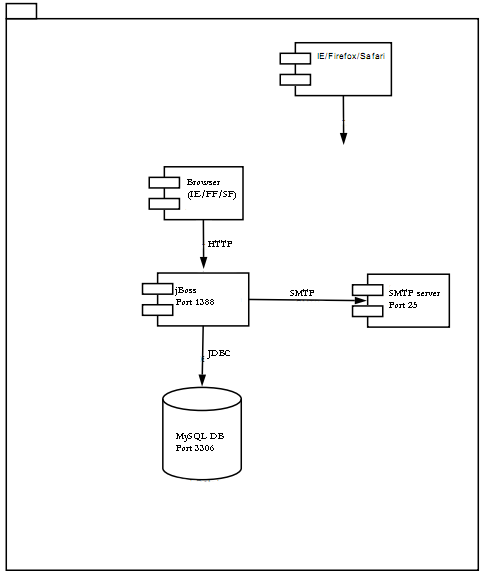
\includegraphics[scale=0.8]{../../img/archi1.png}
\caption{Salesmen Architecture}
\end{figure}

\begin{figure}
\section{Infrastructure}
\label{fig_infrastructure}
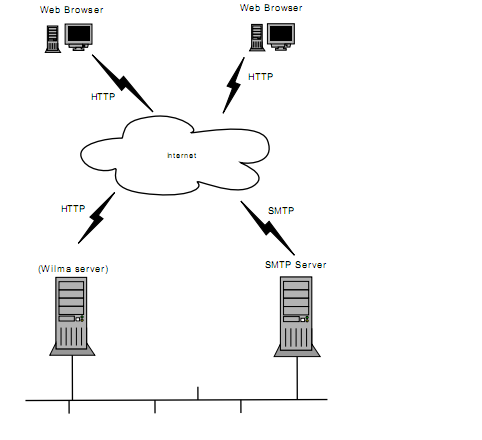
\includegraphics[scale=0.8]{../../img/infra1.png}
\caption{Salesmen infrastructure}
\end{figure}

\begin{figure}
\section{Class Diagram}
\label{fig_class}
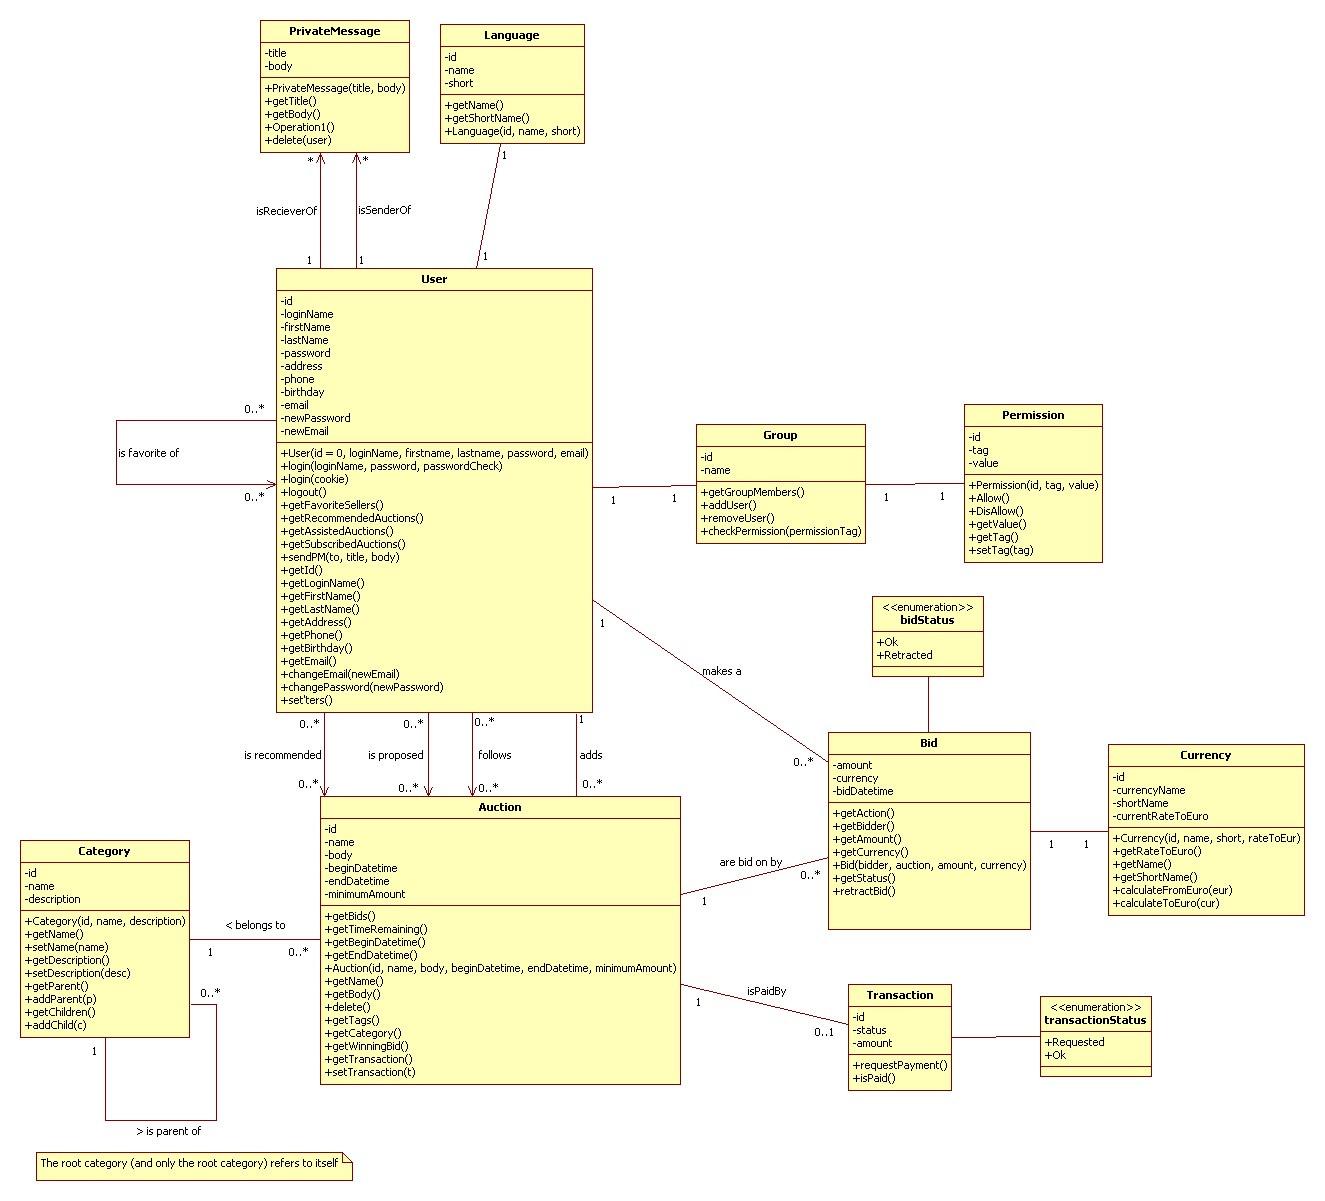
\includegraphics[scale=0.4,angle=90]{../../img/class1.jpg}
\caption{Salesmen class diagram}
\end{figure}

\begin{figure}
\section{Database diagram}
\label{fig_database}
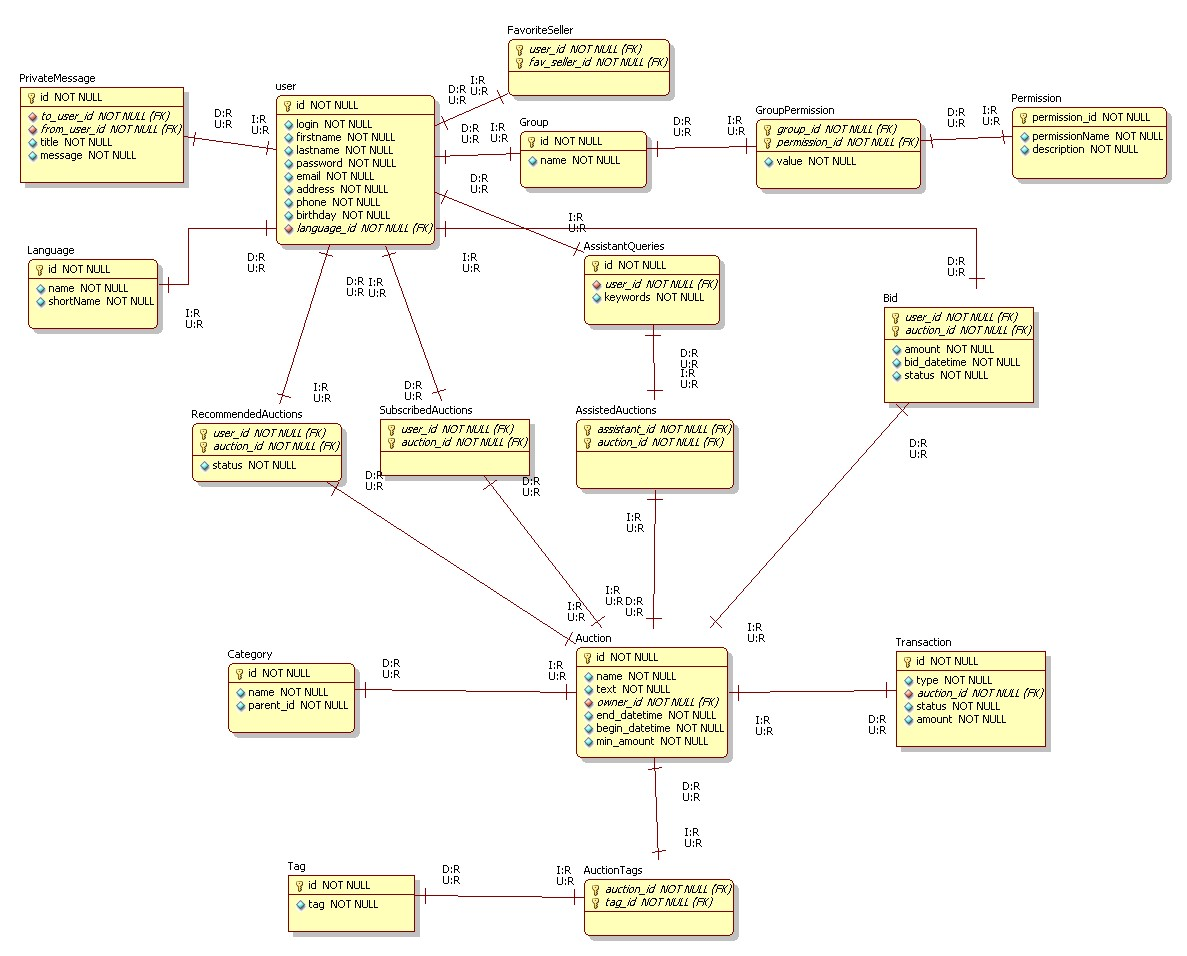
\includegraphics[scale=0.5,angle=90]{../../img/erd1.jpg}
\caption{Salesmen database layout}
\end{figure}

\chapter{Appendix B}
\begin{figure}
\section{Auction list}
\label{fig_prototype_auctionlist}
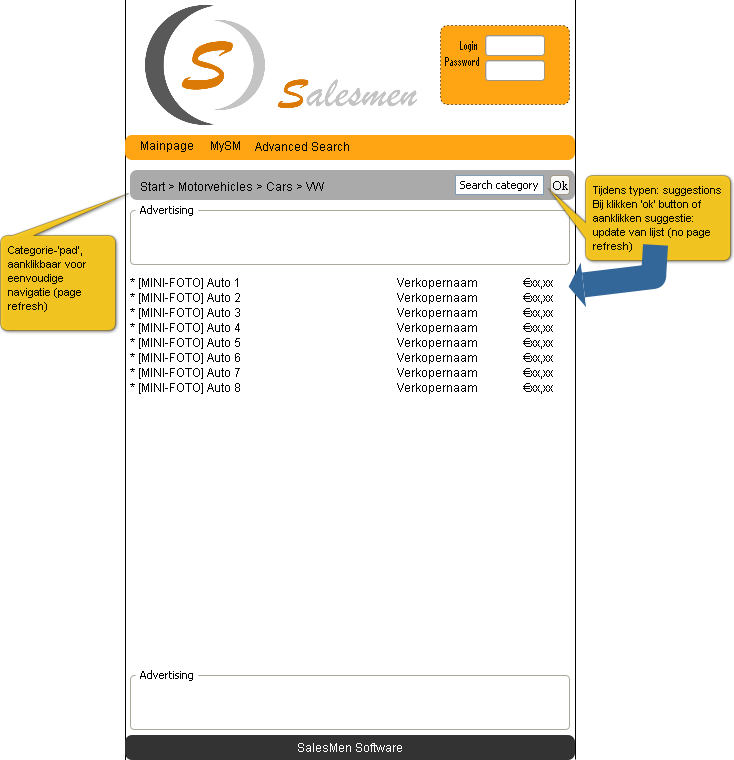
\includegraphics[width=15cm]{../../img/SM_auction_list.png}
\caption{auctionlist.jsp}
\end{figure}
\begin{figure}
\section{Auction detail}
\label{fig_prototype_auctiondetail}
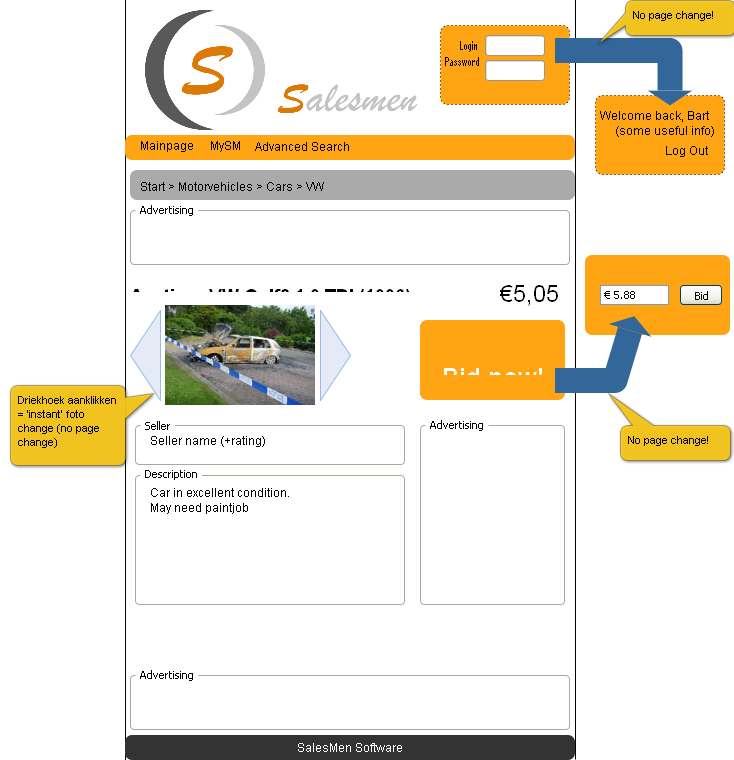
\includegraphics[width=15cm]{../../img/SM_auction_detail.png}
\caption{auctiondetail.jsp}
\end{figure}
\begin{figure}
\section{Profile - Auctions}
\label{fig_prototype_profile_auctions}
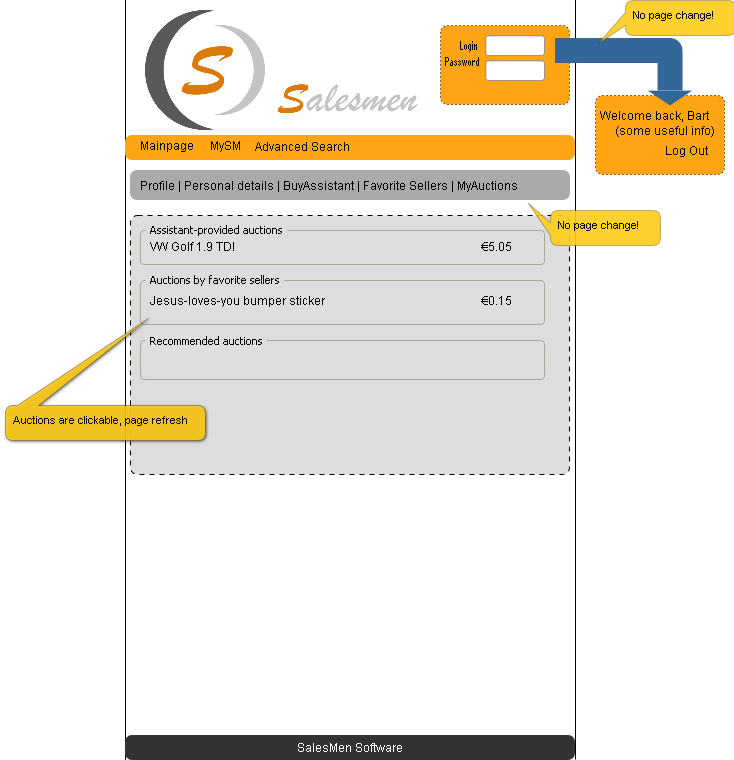
\includegraphics[width=15cm]{../../img/SM_mySM_auctions.png}
\caption{profile.jsp - auctions}
\end{figure}
\begin{figure}
\section{Profile - Buyers assistant}
\label{fig_prototype_buyer_assistant}
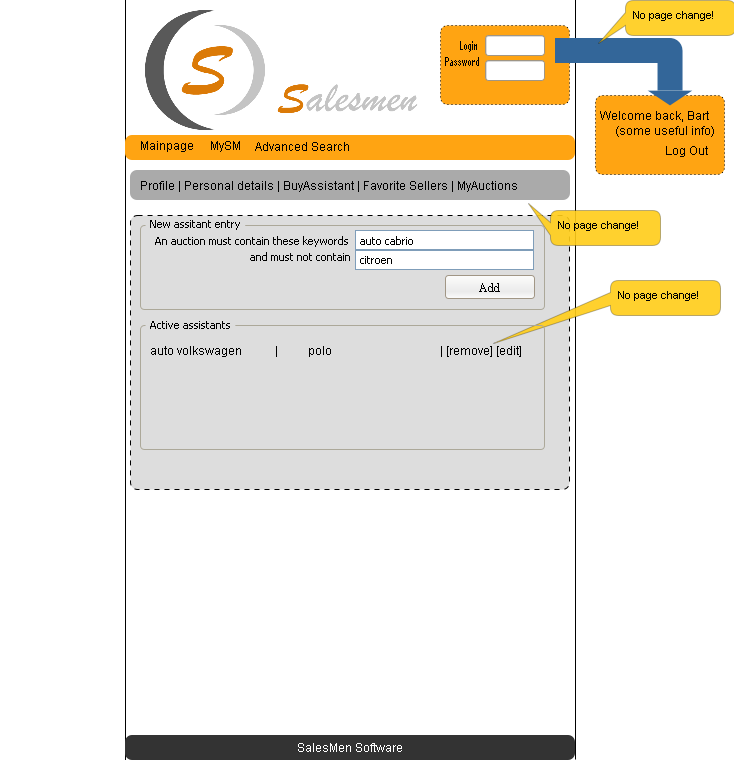
\includegraphics[width=15cm]{../../img/SM_mySM_buy_assistant.png}
\caption{profile.jsp - buyers assistant}
\end{figure}
\begin{figure}
\section{Profile - Personal information}
\label{fig_prototype_personal_info}
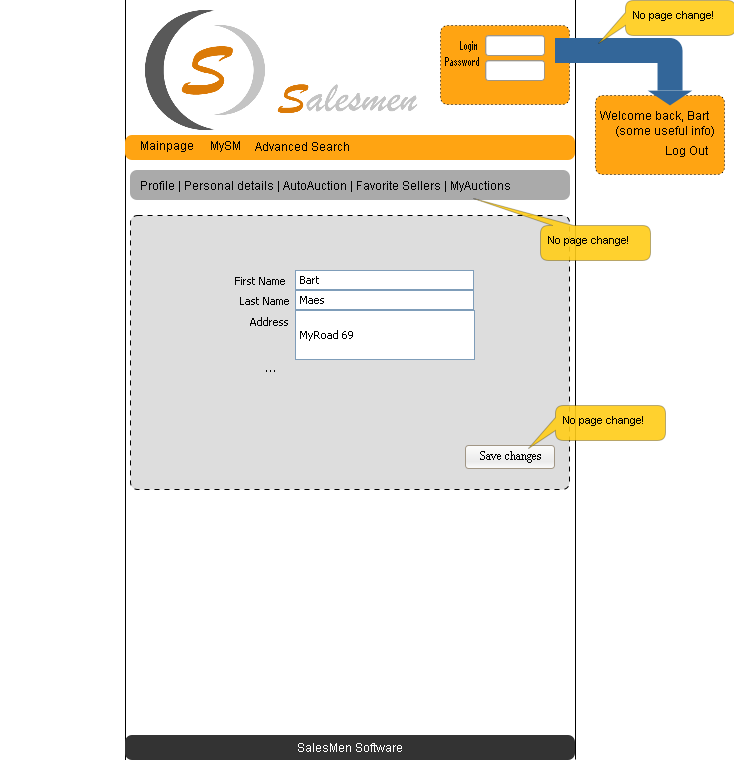
\includegraphics[width=15cm]{../../img/SM_mySM_personal.png}
\caption{profile.jsp - personal information}
\end{figure}
\begin{figure}
\section{Profile - Account information}
\label{fig_prototype_account_info}
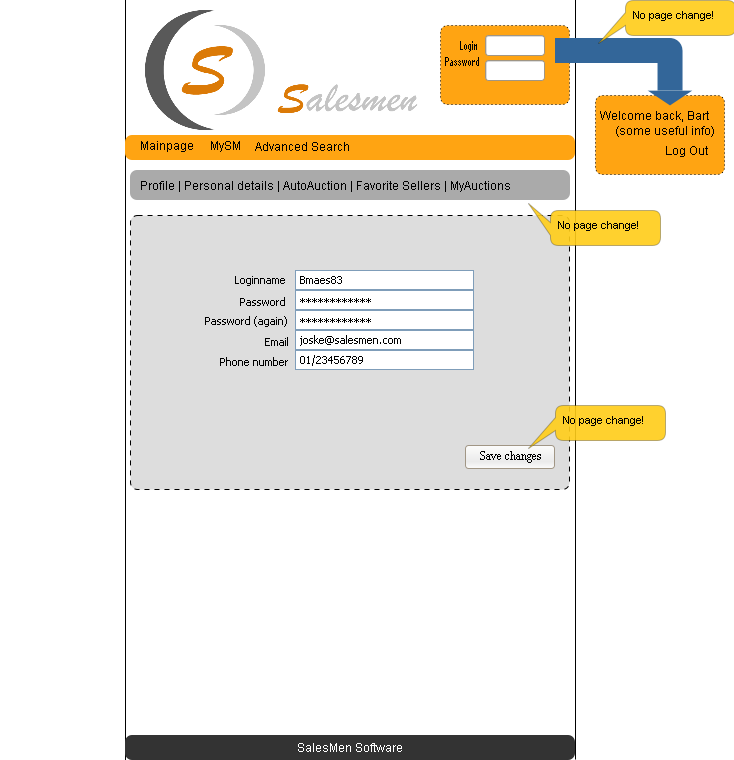
\includegraphics[width=15cm]{../../img/SM_mySM_profile.png}
\caption{profile.jsp - website information}
\end{figure}

\end{document}
